\subsection{Segmentacja semantyczna}
Używając biblioteki \textit{PyTorch} do uczenia głębokiego, w oparciu o istniejące rozwiązania i aktualny stan wiedzy, przygotowano i wytrenowano własne modele \emph{sieci neuronowych} do segmentacji semantycznej, korzystając z modelu \textit{PointNet}\cite{pointnet}, bazując na gotowych implementacjach\cite{Pytorch_Pointnet_Pointnet2}.
W toku eksperymentów ze sposobami implementacji procesu treningu i predykcji za kluczowe pod względem wpływu na osiągi otrzymanego modelu należy uznać:
\begin{enumerate}
    \item próbkowanie - przy przetwarzaniu zbiorów danych, w przypadku których określenie porządku jest z punktu widzenia efektywności rozwiązania bezcelowe lub niemożliwe, a które jednocześnie z punktu widzenia modelu mogą osiągać różne rozmiary, ważnym elementem procesu zarówno treningu, jak i predykcji jest odpowiednie próbkowanie całego zbioru. W obrębie tego problemu należy wyróżnić następujące czynniki:
    \begin{enumerate}
        \item rozmiar próbki - zbyt mały może uniemożliwić uchwycenie zależności pomiędzy zbliżonymi do siebie w chmurze punktami,
        \item sposób próbkowania - wpływa na zależność uchwyconych w wyniku procesu uczenia wzorców od bardziej lub mniej odległych od siebie punktów. Może prowadzić do swego rodzaju zdominowania segmentowanych punktów przez jedną kategorię.
    \end{enumerate}
    \item niezbalansowany zbiór danych - w przypadku rozpatrywania dużych scen miejskich naturalnym jest pojawienie się mniej (\textit{samochody}, \textit{tory kolejowe}) i bardziej (\textit{budynki}) popularnych kategorii semantycznych. Jest to klasyczny problem uczenia maszynowego na niezbalansowanym zbiorze danych, który, niezaadresowany, prowadzi do dominacji zbioru przez punkty popularniejszych kategorii, w efekcie przekładając się na słabszą generalizację otrzymanego modelu, w szczególności dla mniej popularnych kategorii semantycznych. W toku prac rozważano dwa sposoby radzenia sobie z tym problemem:
    \begin{enumerate}
        \item próbkowanie - opisane wyżej,
        \item ważenie funkcji straty - \textit{karze} model za omijanie mniej popularnych kategorii semantycznych. Technika ta może prowadzić do nadreprezentacji tych kategorii w otrzymanym w wyniku predykcji zbiorze, jednakże przy odpowiedniej implementacji nieco słabsze wartości metryk dla popularnych kategorii są \textit{nomen omen} balansowane przez lepsze wyniki na niedoreprezentowanych w zbiorze treningowym kategorii, prowadząc w efekcie do lepszych wartości metryk dla całego zbioru testowego.
    \end{enumerate}
    \item dobór danych treningowych, walidacyjnych i testowych - typowy problem dla uczenia maszynowego. Dbając o generalizację modelu nie możemy dopuścić do \textit{wycieku danych}, tj. sytuacji, w której obiecujące wyniki są spowodowane nie ową generalizacją, a pewnego rodzaju pokrewieństwem danych służących do treningu modelu i jego oceny w trakcie tego procesu lub po jego zakończeniu. Rozwązaniem oprócz odpowiedniego podziału i doboru danych jest użycie technik przetwarzania chmur punktów związanych np. z ich obracaniem lub skalowaniem, tak aby wyuczone wzorce podlegały jak najlepszemu uogólnieniu.
\end{enumerate}

\begin{figure}[!h]
    \centering
    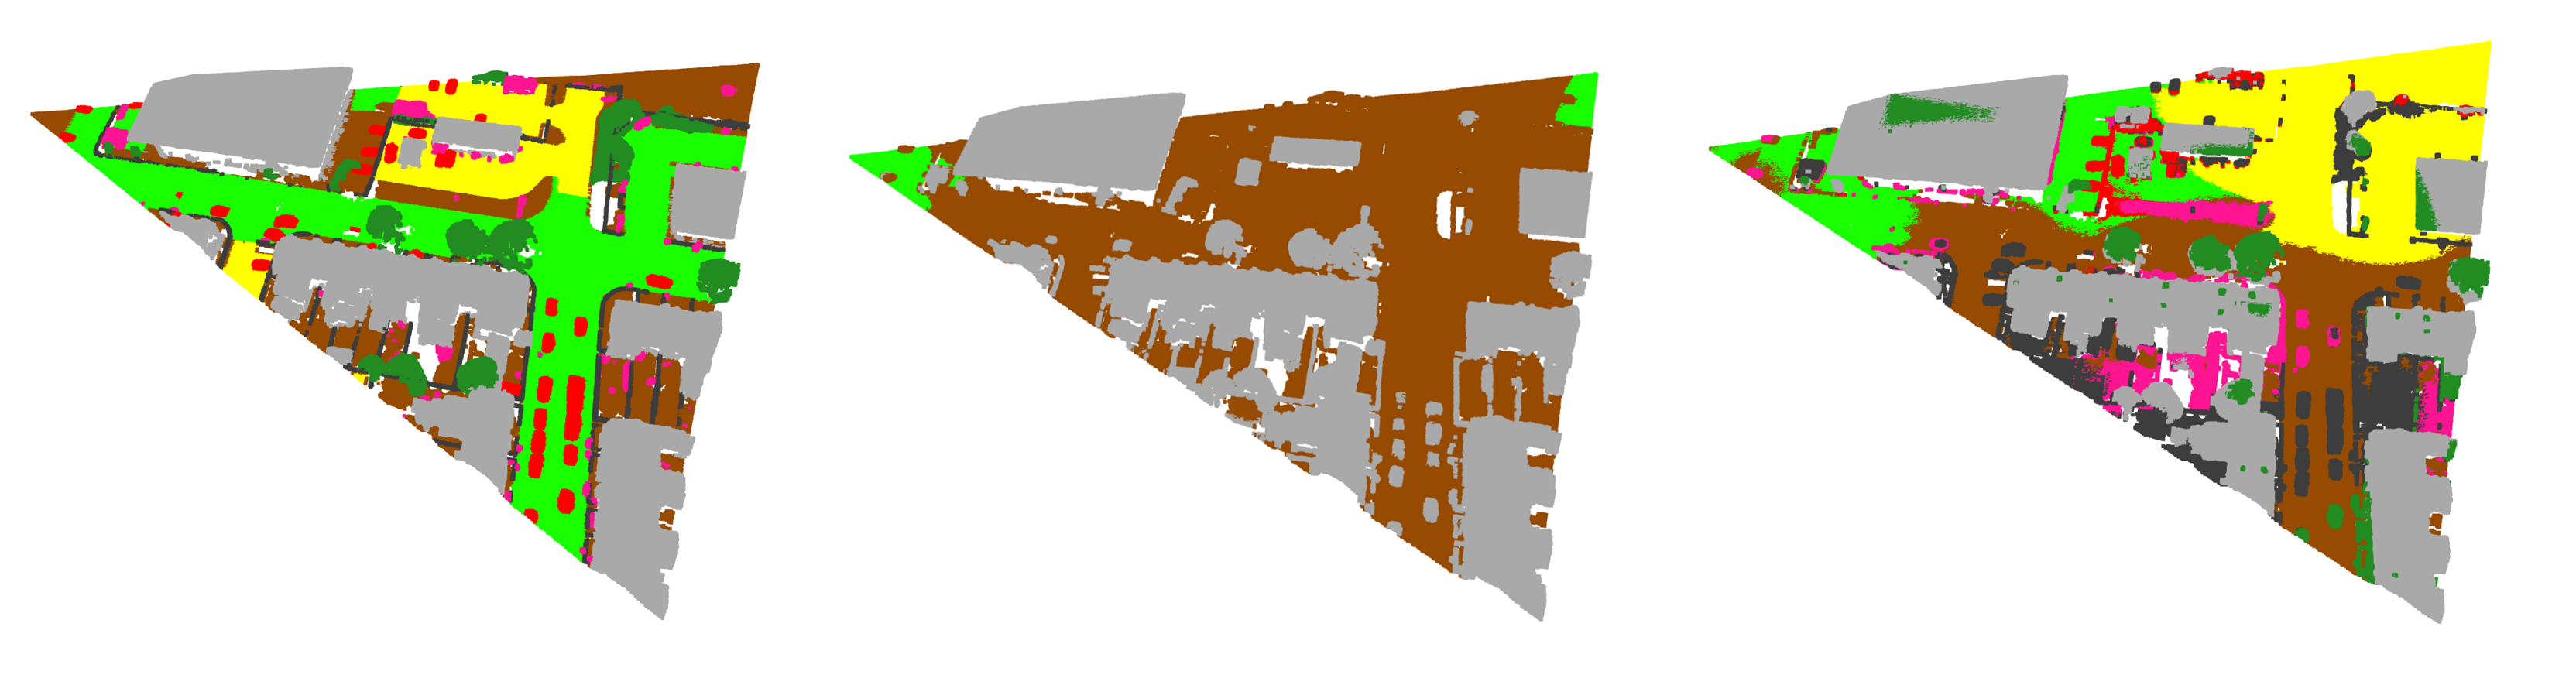
\includegraphics[width=1.0\linewidth]{img/segmentacja/weighted_loss.png}
    \caption{Kolejno: \textit{ground truth}, predykcja modelu bez ważenia funkcji straty i predykcja modelu ważącego funkcję straty.}
    \label{fig:seg_wei}
\end{figure}

Na podstawie badań jakościowych\ref{fig:seg_wei} i \ref{table:tab_seg_met} ilościowych działania modeli nieważących i ważących funkcję straty stwierdzono poprawę metryk oddających osiągi w predykcji klas słabiej reprezentowanych. Model z ważoną funkcją straty może jednak osiągać słabsze wyniki na klasach najliczniejszych, doszukując się w ich reprezentantach przedstawicieli klas mniej licznych, których niedopatrywanie w procesie treningu było w związku z ważeniem funkcji kosztu odgrywało większą rolę w procesie propagacji wstecznej.

Do trenowania posłużyliśmy się zbiorem \textit{SensatUrban}\cite{hu2022sensaturban}, często używanym w literaturze do oceny modeli segmentacji semantycznej.

\begin{table}[!h]
    \centering
    \begin{tabular}{|c|c|c|c|c|c|c|c|c|c|}
    \hline
    WL & TS & OwAcc & OwF & budAcc & budkF & zieAcc & zieF & parAcc & parF \\
    \hline 
    Nie & 238 950 & 43.37 & 37.50 & 83 & \textbf{87} & 0 & 0 & \textbf{51} & 11 \\
    \hline 
    Nie & 19 509 208 & 31.68 & 30.57 & 52 & 54 & 13 & 2 & 15 & 7 \\
    \hline 
    Tak & 238 950 & \textbf{50.69} & \textbf{45.57} & \textbf{91} & 84 & \textbf{42} & \textbf{38} & 44 & \textbf{28} \\
    \hline
    Tak & 19 509 208 & 31.72 & 17.89 & 52 & 24 & 13 & 19 & 15 & 15 \\
    \hline
    \end{tabular}
\caption{Metryki dla eksperymentów z modelami \textit{PointNet}. Ważenie funkcji straty, rozmiar zbioru testowego, całkowita ważona dokładność, całkowity ważony F-score, dokładność i F-score dla kategorii: \textit{budynek}, \textit{teren zielony} i \textit{parking}.}
\label{table:tab_seg_met}
\end{table}

Otrzymany w wyniku tego procesu eksperymentowania model wdrożono w celu jego używania na \textit{niewidzianych} przez niego dotychczas danych.